\documentclass[letterpaper]{article}
\usepackage{tikz}
\usetikzlibrary{arrows,shapes,automata,petri,positioning,calc}
\tikzset{
    nodeStyle/.style={
        circle,
        thick,
        draw=black,
        fill=white!30,
        minimum size=3mm,
    },
    nodeStyleIncDec/.style={
        circle,
        thick,
        draw=black,
        fill=white!30,
        minimum size=8mm,
    },
    posStyle/.style={
        circle,
        thick,
        draw=black,
        fill=green!30,
        minimum size=8mm,
    },
    negStyle/.style={
        circle,
        thick,
        draw=black,
        fill=red!30,
        minimum size=8mm,
    },
    dottedRectangle/.style={dashed},
}

\begin{document}

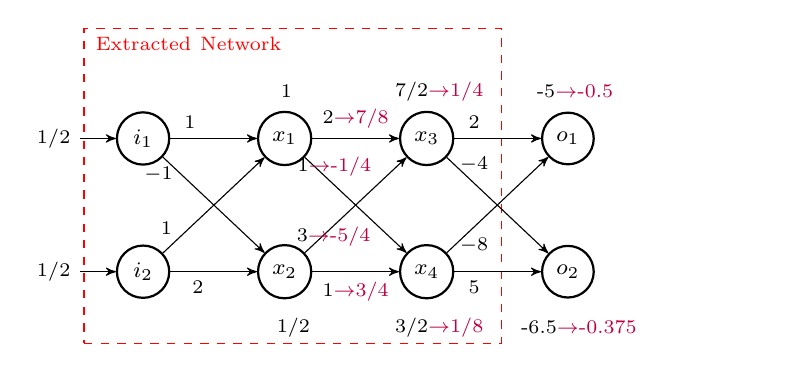
\begin{tikzpicture}[node distance=1cm and 1.1cm,>=stealth',auto,initial text={\scriptsize $1/2$}, every place/.style={draw}]
        
        \node[rectangle, dottedRectangle,
        draw = red,
        text = red,
        minimum width = 5.3cm, 
        align=left,
        minimum height = 4cm] (r) at (1.9,-0.6) {};
        \node[text width=3cm] at (0.9,1.2) {\textcolor{red}{\scriptsize Extracted Network}};
        
        \node[text width=3cm] at (3.2,-2.4) {\scriptsize 1/2};
        \node[text width=3cm] at (4.7,-2.4) {\scriptsize 3/2\textcolor{purple}{$\rightarrow$1/8}};
        \node[text width=3cm] at (6.3,-2.4) {\scriptsize -6.5\textcolor{purple}{$\rightarrow$-0.375}};
        \node[text width=3cm] at (3.25,0.6) {\scriptsize 1};
        \node[text width=3cm] at (4.7,0.6) {\scriptsize 7/2\textcolor{purple}{$\rightarrow$1/4}};
        \node[text width=3cm] at (6.5,0.6) {\scriptsize -5\textcolor{purple}{$\rightarrow$-0.5}};
        

		\node [nodeStyle,initial] (i1) {\footnotesize $i_{1}$};
		\node [nodeStyle,initial] (i2) [below=of i1] {\footnotesize $i_{2}$};
		\node [nodeStyle] (x1) [right=of i1] {\footnotesize $x_{1}$};
		\node [nodeStyle] (x2) [right=of i2] {\footnotesize $x_{2}$};
		\node [nodeStyle] (x3) [right=of x1] {\footnotesize $x_{3}$};
		\node [nodeStyle] (x4) [right=of x2] {\footnotesize $x_{4}$};
		\node [nodeStyle] (o1) [right=of x3] {\footnotesize $o_{1}$};
		\node [nodeStyle] (o2) [right=of x4] {\footnotesize $o_{2}$};
		
		\path[->] (i1) edge node[above, xshift=-0.3cm, yshift=0cm] {\scriptsize $1$} (x1);
		\path[->] (i2) edge node[below, xshift=-0.2cm, yshift=0cm] {\scriptsize $2$} (x2);
		\path[->] (i1) edge node[below, xshift=-0.7cm, yshift=0.6cm] {\scriptsize $-1$} (x2);
		\path[->] (i2) edge node[above, xshift=-0.6cm, yshift=-0.5cm] {\scriptsize $1$} (x1);
		\path[->] (x1) edge node[above, xshift=0cm, yshift=0cm] {\scriptsize 2\textcolor{purple}{$\rightarrow$7/8}} (x3);
		\path[->] (x2) edge node[below, xshift=0cm, yshift=0cm] {\scriptsize 1\textcolor{purple}{$\rightarrow$3/4}} (x4);
		\path[->] (x2) edge node[above, xshift=-0.28cm, yshift=-0.65cm] {\scriptsize 3\textcolor{purple}{$\rightarrow$-5/4}} (x3);
		\path[->] (x1) edge node[above, xshift=-0.27cm, yshift=0.24cm] {\scriptsize 1\textcolor{purple}{$\rightarrow$-1/4}} (x4);
		\path[->] (x3) edge node[above, xshift=-0.3cm, yshift=0cm] {\scriptsize $2$} (o1);
		\path[->] (x4) edge node[below, xshift=-0.3cm, yshift=0cm] {\scriptsize $5$} (o2);
		\path[->] (x3) edge node[above, xshift=-0.3cm, yshift=0.3cm] {\scriptsize $-4$} (o2);
		\path[->] (x4) edge node[below, xshift=-0.3cm, yshift=-0.3cm] {\scriptsize $-8$} (o1);
	\end{tikzpicture}

\end{document}